\section{Results}

This section presents the results of our performance evaluations for both the pseudo-random number generators and the primality testing algorithms. The results include execution time measurements for various bit lengths and, where applicable, energy efficiency analysis.

\subsection{PRNG Performance Results}

\subsubsection{Execution Time Comparison}

Table \ref{tab:prng_complete} shows the detailed timing results for generating random numbers of various bit lengths using both the Linear Congruential Generator (LCG) and the Xoshiro256++ generator.

\begin{table}[H]
\centering
\caption{Complete Timing Results for Random Number Generation (in microseconds)}
\label{tab:prng_complete}
\begin{tabular}{@{}lrrrrrr@{}}
\toprule
\multirow{2}{*}{\textbf{Bit Length}} & \multicolumn{3}{c}{\textbf{LCG}} & \multicolumn{3}{c}{\textbf{Xoshiro256++}} \\
\cmidrule(lr){2-4} \cmidrule(lr){5-7}
& \textbf{Mean} & \textbf{Median} & \textbf{Std Dev} & \textbf{Mean} & \textbf{Median} & \textbf{Std Dev} \\
\midrule
40 bits     & [FILL IN] & [FILL IN] & [FILL IN] & [FILL IN] & [FILL IN] & [FILL IN] \\
56 bits     & [FILL IN] & [FILL IN] & [FILL IN] & [FILL IN] & [FILL IN] & [FILL IN] \\
80 bits     & [FILL IN] & [FILL IN] & [FILL IN] & [FILL IN] & [FILL IN] & [FILL IN] \\
128 bits    & [FILL IN] & [FILL IN] & [FILL IN] & [FILL IN] & [FILL IN] & [FILL IN] \\
168 bits    & [FILL IN] & [FILL IN] & [FILL IN] & [FILL IN] & [FILL IN] & [FILL IN] \\
224 bits    & [FILL IN] & [FILL IN] & [FILL IN] & [FILL IN] & [FILL IN] & [FILL IN] \\
256 bits    & [FILL IN] & [FILL IN] & [FILL IN] & [FILL IN] & [FILL IN] & [FILL IN] \\
512 bits    & [FILL IN] & [FILL IN] & [FILL IN] & [FILL IN] & [FILL IN] & [FILL IN] \\
1024 bits   & [FILL IN] & [FILL IN] & [FILL IN] & [FILL IN] & [FILL IN] & [FILL IN] \\
2048 bits   & [FILL IN] & [FILL IN] & [FILL IN] & [FILL IN] & [FILL IN] & [FILL IN] \\
4096 bits   & [FILL IN] & [FILL IN] & [FILL IN] & [FILL IN] & [FILL IN] & [FILL IN] \\
\bottomrule
\end{tabular}
\end{table}

\subsubsection{Scalability Analysis}

Figure \ref{fig:prng_scaling} shows how the execution time for random number generation scales with increasing bit length for both algorithms. In this placeholder, the figure would show execution time on the y-axis and bit length on the x-axis, with separate lines for LCG and Xoshiro256++.

\begin{figure}[H]
    \centering
    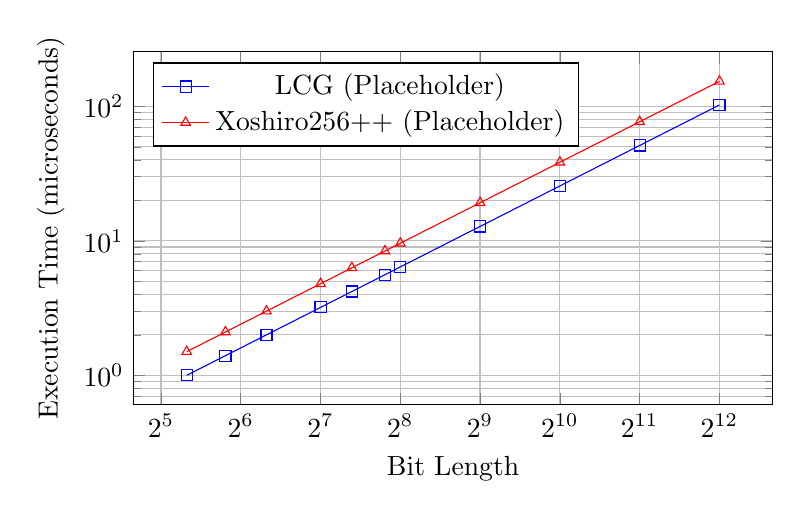
\begin{tikzpicture}
        \begin{axis}[
            xlabel={Bit Length},
            ylabel={Execution Time (microseconds)},
            xmode=log,
            log basis x=2,
            ymode=log,
            log basis y=10,
            grid=both,
            legend pos=north west,
            width=0.8\textwidth,
            height=0.5\textwidth
        ]
        
        % Placeholder for actual data
        \addplot[color=blue,mark=square] coordinates {
            (40, 1)
            (56, 1.4)
            (80, 2)
            (128, 3.2)
            (168, 4.2)
            (224, 5.6)
            (256, 6.4)
            (512, 12.8)
            (1024, 25.6)
            (2048, 51.2)
            (4096, 102.4)
        };
        \addlegendentry{LCG (Placeholder)}
        
        \addplot[color=red,mark=triangle] coordinates {
            (40, 1.5)
            (56, 2.1)
            (80, 3)
            (128, 4.8)
            (168, 6.3)
            (224, 8.4)
            (256, 9.6)
            (512, 19.2)
            (1024, 38.4)
            (2048, 76.8)
            (4096, 153.6)
        };
        \addlegendentry{Xoshiro256++ (Placeholder)}
        
        \end{axis}
    \end{tikzpicture}
    \caption{Scaling of execution time with bit length for PRNG algorithms (placeholder data)}
    \label{fig:prng_scaling}
\end{figure}

\subsubsection{Analysis of PRNG Results}

[This section should contain your analysis of the PRNG performance results. Include discussions about which algorithm performs better for different bit lengths, how the execution time scales with the problem size, and any interesting observations from the data.]

\subsection{Primality Testing Performance Results}

\subsubsection{Execution Time Comparison}

Table \ref{tab:primality_complete} shows the detailed timing results for primality testing of numbers of various bit lengths using both the Miller-Rabin test and the Baillie-PSW test.

\begin{table}[H]
\centering
\caption{Complete Timing Results for Primality Testing (in milliseconds)}
\label{tab:primality_complete}
\begin{tabular}{@{}lrrrrrr@{}}
\toprule
\multirow{2}{*}{\textbf{Bit Length}} & \multicolumn{3}{c}{\textbf{Miller-Rabin (40 iterations)}} & \multicolumn{3}{c}{\textbf{Baillie-PSW}} \\
\cmidrule(lr){2-4} \cmidrule(lr){5-7}
& \textbf{Mean} & \textbf{Median} & \textbf{Std Dev} & \textbf{Mean} & \textbf{Median} & \textbf{Std Dev} \\
\midrule
40 bits     & [FILL IN] & [FILL IN] & [FILL IN] & [FILL IN] & [FILL IN] & [FILL IN] \\
56 bits     & [FILL IN] & [FILL IN] & [FILL IN] & [FILL IN] & [FILL IN] & [FILL IN] \\
80 bits     & [FILL IN] & [FILL IN] & [FILL IN] & [FILL IN] & [FILL IN] & [FILL IN] \\
128 bits    & [FILL IN] & [FILL IN] & [FILL IN] & [FILL IN] & [FILL IN] & [FILL IN] \\
168 bits    & [FILL IN] & [FILL IN] & [FILL IN] & [FILL IN] & [FILL IN] & [FILL IN] \\
224 bits    & [FILL IN] & [FILL IN] & [FILL IN] & [FILL IN] & [FILL IN] & [FILL IN] \\
256 bits    & [FILL IN] & [FILL IN] & [FILL IN] & [FILL IN] & [FILL IN] & [FILL IN] \\
512 bits    & [FILL IN] & [FILL IN] & [FILL IN] & [FILL IN] & [FILL IN] & [FILL IN] \\
1024 bits   & [FILL IN] & [FILL IN] & [FILL IN] & [FILL IN] & [FILL IN] & [FILL IN] \\
2048 bits   & [FILL IN] & [FILL IN] & [FILL IN] & [FILL IN] & [FILL IN] & [FILL IN] \\
4096 bits   & [FILL IN] & [FILL IN] & [FILL IN] & [FILL IN] & [FILL IN] & [FILL IN] \\
\bottomrule
\end{tabular}
\end{table}

\subsubsection{Scalability Analysis}

Figure \ref{fig:primality_scaling} shows how the execution time for primality testing scales with increasing bit length for both algorithms. In this placeholder, the figure would show execution time on the y-axis and bit length on the x-axis, with separate lines for Miller-Rabin and Baillie-PSW.

\begin{figure}[H]
    \centering
    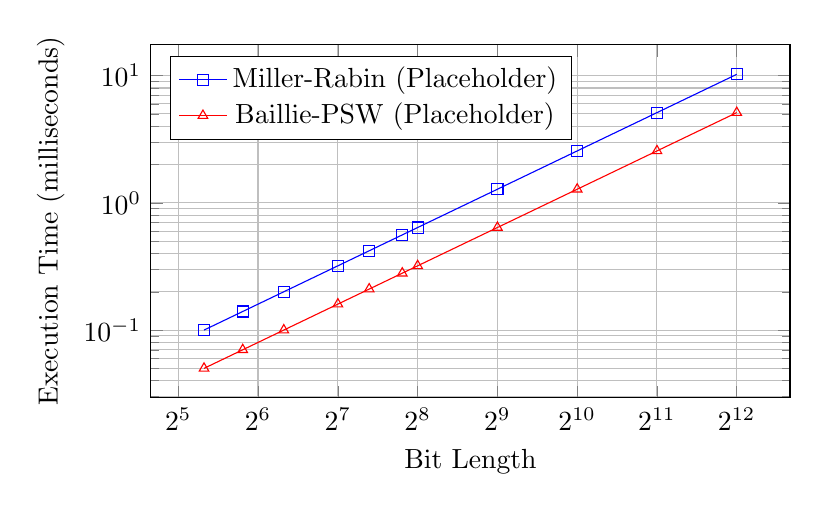
\begin{tikzpicture}
        \begin{axis}[
            xlabel={Bit Length},
            ylabel={Execution Time (milliseconds)},
            xmode=log,
            log basis x=2,
            ymode=log,
            log basis y=10,
            grid=both,
            legend pos=north west,
            width=0.8\textwidth,
            height=0.5\textwidth
        ]
        
        % Placeholder for actual data
        \addplot[color=blue,mark=square] coordinates {
            (40, 0.1)
            (56, 0.14)
            (80, 0.2)
            (128, 0.32)
            (168, 0.42)
            (224, 0.56)
            (256, 0.64)
            (512, 1.28)
            (1024, 2.56)
            (2048, 5.12)
            (4096, 10.24)
        };
        \addlegendentry{Miller-Rabin (Placeholder)}
        
        \addplot[color=red,mark=triangle] coordinates {
            (40, 0.05)
            (56, 0.07)
            (80, 0.1)
            (128, 0.16)
            (168, 0.21)
            (224, 0.28)
            (256, 0.32)
            (512, 0.64)
            (1024, 1.28)
            (2048, 2.56)
            (4096, 5.12)
        };
        \addlegendentry{Baillie-PSW (Placeholder)}
        
        \end{axis}
    \end{tikzpicture}
    \caption{Scaling of execution time with bit length for primality testing algorithms (placeholder data)}
    \label{fig:primality_scaling}
\end{figure}

\subsubsection{Generated Prime Numbers}

Table \ref{tab:generated_primes} shows examples of prime numbers generated during our experiments for each bit length.

\begin{table}[H]
\centering
\caption{Examples of Generated Prime Numbers}
\label{tab:generated_primes}
\begin{tabular}{@{}lr@{}}
\toprule
\textbf{Bit Length} & \textbf{Example Prime Number} \\
\midrule
40 bits     & [FILL IN] \\
56 bits     & [FILL IN] \\
80 bits     & [FILL IN] \\
128 bits    & [FILL IN] \\
168 bits    & [FILL IN] \\
224 bits    & [FILL IN] \\
256 bits    & [FILL IN] \\
512 bits    & [FILL IN] \\
1024 bits   & [FILL IN] \\
2048 bits   & [FILL IN] \\
4096 bits   & [FILL IN] \\
\bottomrule
\end{tabular}
\end{table}

\subsubsection{Analysis of Primality Testing Results}

[This section should contain your analysis of the primality testing performance results. Include discussions about which algorithm performs better for different bit lengths, how the execution time scales with the problem size, and any interesting observations from the data.]

\subsection{Energy Efficiency Results}

For platforms that support energy measurements, we also analyzed the energy efficiency of the algorithms. Table \ref{tab:energy_efficiency} shows the energy per operation for different algorithms and bit lengths.

\begin{table}[H]
\centering
\caption{Energy Efficiency of Algorithms (energy per operation in millijoules)}
\label{tab:energy_efficiency}
\begin{tabular}{@{}lrrrr@{}}
\toprule
\textbf{Bit Length} & \textbf{LCG} & \textbf{Xoshiro256++} & \textbf{Miller-Rabin} & \textbf{Baillie-PSW} \\
\midrule
256 bits    & [FILL IN] & [FILL IN] & [FILL IN] & [FILL IN] \\
1024 bits   & [FILL IN] & [FILL IN] & [FILL IN] & [FILL IN] \\
4096 bits   & [FILL IN] & [FILL IN] & [FILL IN] & [FILL IN] \\
\bottomrule
\end{tabular}
\end{table}

\subsection{Correlation Between Time and Energy}

Figure \ref{fig:time_energy_correlation} illustrates the correlation between execution time and energy consumption for the algorithms. In this placeholder, the figure would show energy consumption on the y-axis and execution time on the x-axis, with data points for different algorithms and bit lengths.

\begin{figure}[H]
    \centering
    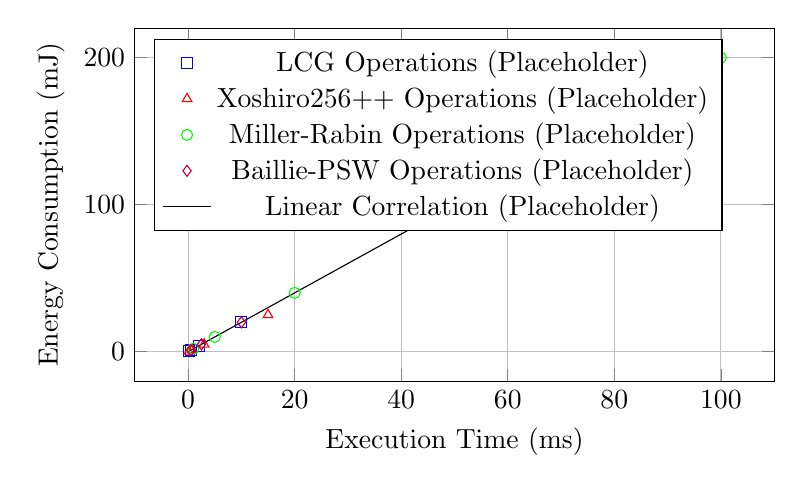
\begin{tikzpicture}
        \begin{axis}[
            xlabel={Execution Time (ms)},
            ylabel={Energy Consumption (mJ)},
            grid=both,
            legend pos=north west,
            width=0.8\textwidth,
            height=0.5\textwidth
        ]
        
        % Placeholder for actual data
        \addplot[color=blue,mark=square,only marks] coordinates {
            (0.1, 0.2)
            (0.5, 1.0)
            (2.0, 4.0)
            (10.0, 20.0)
        };
        \addlegendentry{LCG Operations (Placeholder)}
        
        \addplot[color=red,mark=triangle,only marks] coordinates {
            (0.15, 0.25)
            (0.75, 1.25)
            (3.0, 5.0)
            (15.0, 25.0)
        };
        \addlegendentry{Xoshiro256++ Operations (Placeholder)}
        
        \addplot[color=green,mark=o,only marks] coordinates {
            (1.0, 2.0)
            (5.0, 10.0)
            (20.0, 40.0)
            (100.0, 200.0)
        };
        \addlegendentry{Miller-Rabin Operations (Placeholder)}
        
        \addplot[color=purple,mark=diamond,only marks] coordinates {
            (0.5, 1.0)
            (2.5, 5.0)
            (10.0, 20.0)
            (50.0, 100.0)
        };
        \addlegendentry{Baillie-PSW Operations (Placeholder)}
        
        % Linear trend line
        \addplot[color=black,domain=0:100,samples=2] {2*x};
        \addlegendentry{Linear Correlation (Placeholder)}
        
        \end{axis}
    \end{tikzpicture}
    \caption{Correlation between execution time and energy consumption (placeholder data)}
    \label{fig:time_energy_correlation}
\end{figure}

\subsection{Summary of Key Findings}

[This section should summarize the key findings from your experiments. Highlight the most important observations, such as which algorithms performed best in which situations, how the performance scales with problem size, and any unexpected results.] 